\documentclass[a4paper]{article}
\usepackage{geometry}
\geometry{margin=1in}

\usepackage[english]{babel}
\usepackage[utf8]{inputenc}
\usepackage{amsmath}
\usepackage{graphicx}
\usepackage[colorinlistoftodos]{todonotes}
\usepackage{gensymb}
\usepackage{hyperref}
\usepackage[T1]{fontenc}
\usepackage{lmodern}
\usepackage{minted}
\usepackage{url}
\usepackage{fancyhdr}
\usepackage{wrapfig}

\setlength{\parskip}{0.7em}
\title{ \textbf{Introduction to Programming \& The Internet of Things} \\
Module 1: Basic Circuits \& Elements \vspace{-5ex} \\
}
\date{}

\begin{document}
\maketitle
\thispagestyle{fancy}
\lhead{University of Texas at Austin \\ Civil, Architectural, and Environmental Engineering \\ Material curated by Thomas Dougherty}
\rhead{Professor Dr. Zoltan Nagy \\ https://nagy.caee.utexas.edu \\ Fall 2018}

\section{Modules Background}
There is a pervasive need to study the performance of built structures and their abilities to provide occupants with comfort in an efficient manner. The Internet of Things (IoT) provides methods of obtaining and studying data about our built environments. As such, these modules introduce civil, architectural, and environmental engineers to tropics of electrical engineering. Students will gather the abilities needed to program and deploy necessary sensors in the Internet of Things (IoT), as well as gain the ability to gather and analyze data collected.

\tableofcontents
\newpage

\section{Introduction}
\label{sec:introduction}

Have you ever asked yourself why the lights work? How we're able to determine the temperature of a room? Why we're able to use computers, or even what electricity is? In this module we're going to be exploring the basics of how electricity can be controlled and measured, as well as what these terms mean and what we can learn from them. To start, we'll be talking about voltage and current.

\section{Theory}
\label{sec:theory}

\subsection{Voltage and Current}
Everything is made of atoms. Your heart, your brain, the leaves outside, and the dogs in the park. Often times the more interesting things happen not when atoms are balanced and happy but when they're excited and charged (incidentally, this is the same principle that gave us reality TV). When there's an imbalance in the excitation of particles, this equation describes how their discrepancies relate to the intensity and direction of resulting force: 

\begin{equation} \label{eq:1}
F = \sum{\frac{1}{4\pi\epsilon}\frac{q_{1}q_{2}}{r^2}\hat{r}}
\end{equation}

\vspace{0.5cm}
While this equation is one of the most fundamental theorems about how charged particles interact, it's virtually not used when constructing electrical systems. Instead, we usually think more in terms of Voltage and Current.

\begin{wrapfigure}{l}{0.5\textwidth}
  \begin{center}
    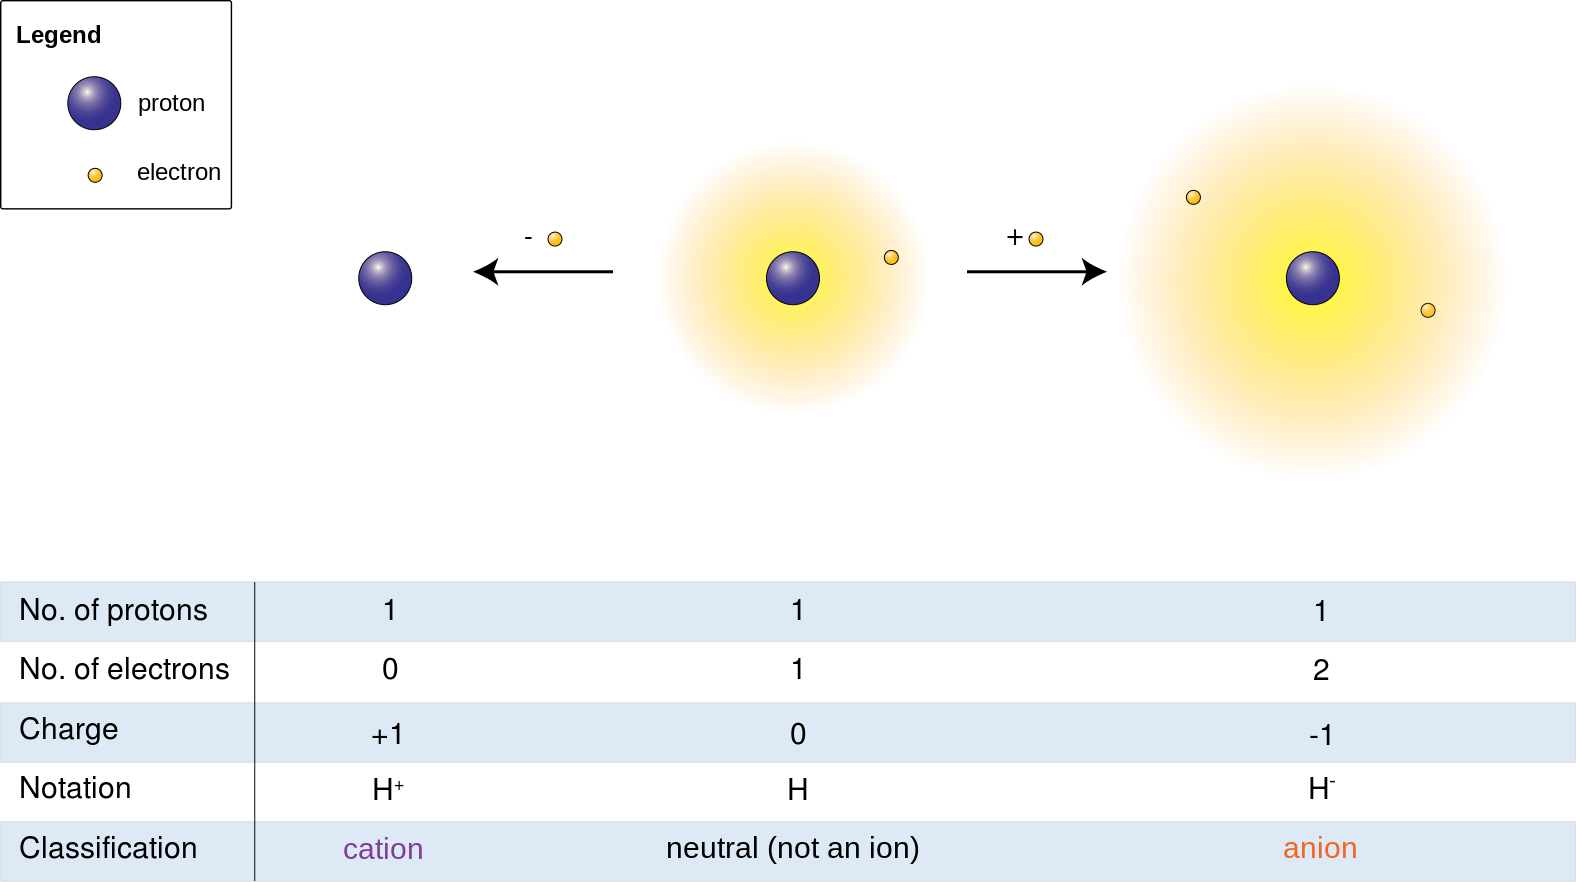
\includegraphics[width=0.5\textwidth]{ions_svg.png}
  \end{center}
  \caption{Ionization Theory}
\end{wrapfigure}

What is Voltage, really? Voltage (V) is technically defined as the difference in electric potential between two points. In layman terms, this means that voltage defines an imbalance in the amount of charge.

Voltage is pretty useful because it allows us to predict how electrons are going to move. Just like we can predict that a ball will roll from the top of a mountain to the bottom of the mountain, we can predict that electrons will flow from a place of high voltage to a place of low voltage. Because of this, we can think of voltage as the driving source of electron movement.

To help understand this, imagine you're in an elevator. When there's nobody around, there's no real motivation to move quickly in and out of this metal box. Now imagine that you're in an elevator with 20 other people. Take note of how quickly you imagine yourself walking out of the elevator, and notice how this is related to the number of people that are in the elevator. The speed at which uncomfortable people (or uncomfortable electrons) leave one place and go to another is called the current (I). Replacing people with charges (Q), we arrive at the formula $I = \frac{dQ}{dt}$ to describe the current.

\subsection{Resistance}
Knowing that voltage drives current (just like your desire to leave a packed elevator drives how quickly you run out of the elevator), how can we relate the two? Regardless of how much you might want to leave, the  speed of flight is limited by the geometry of the elevator. Maybe there's a trash can in the way a pile of rubble.
\newpage
\begin{wrapfigure}{r}{0.4\textwidth}
  \begin{center}
    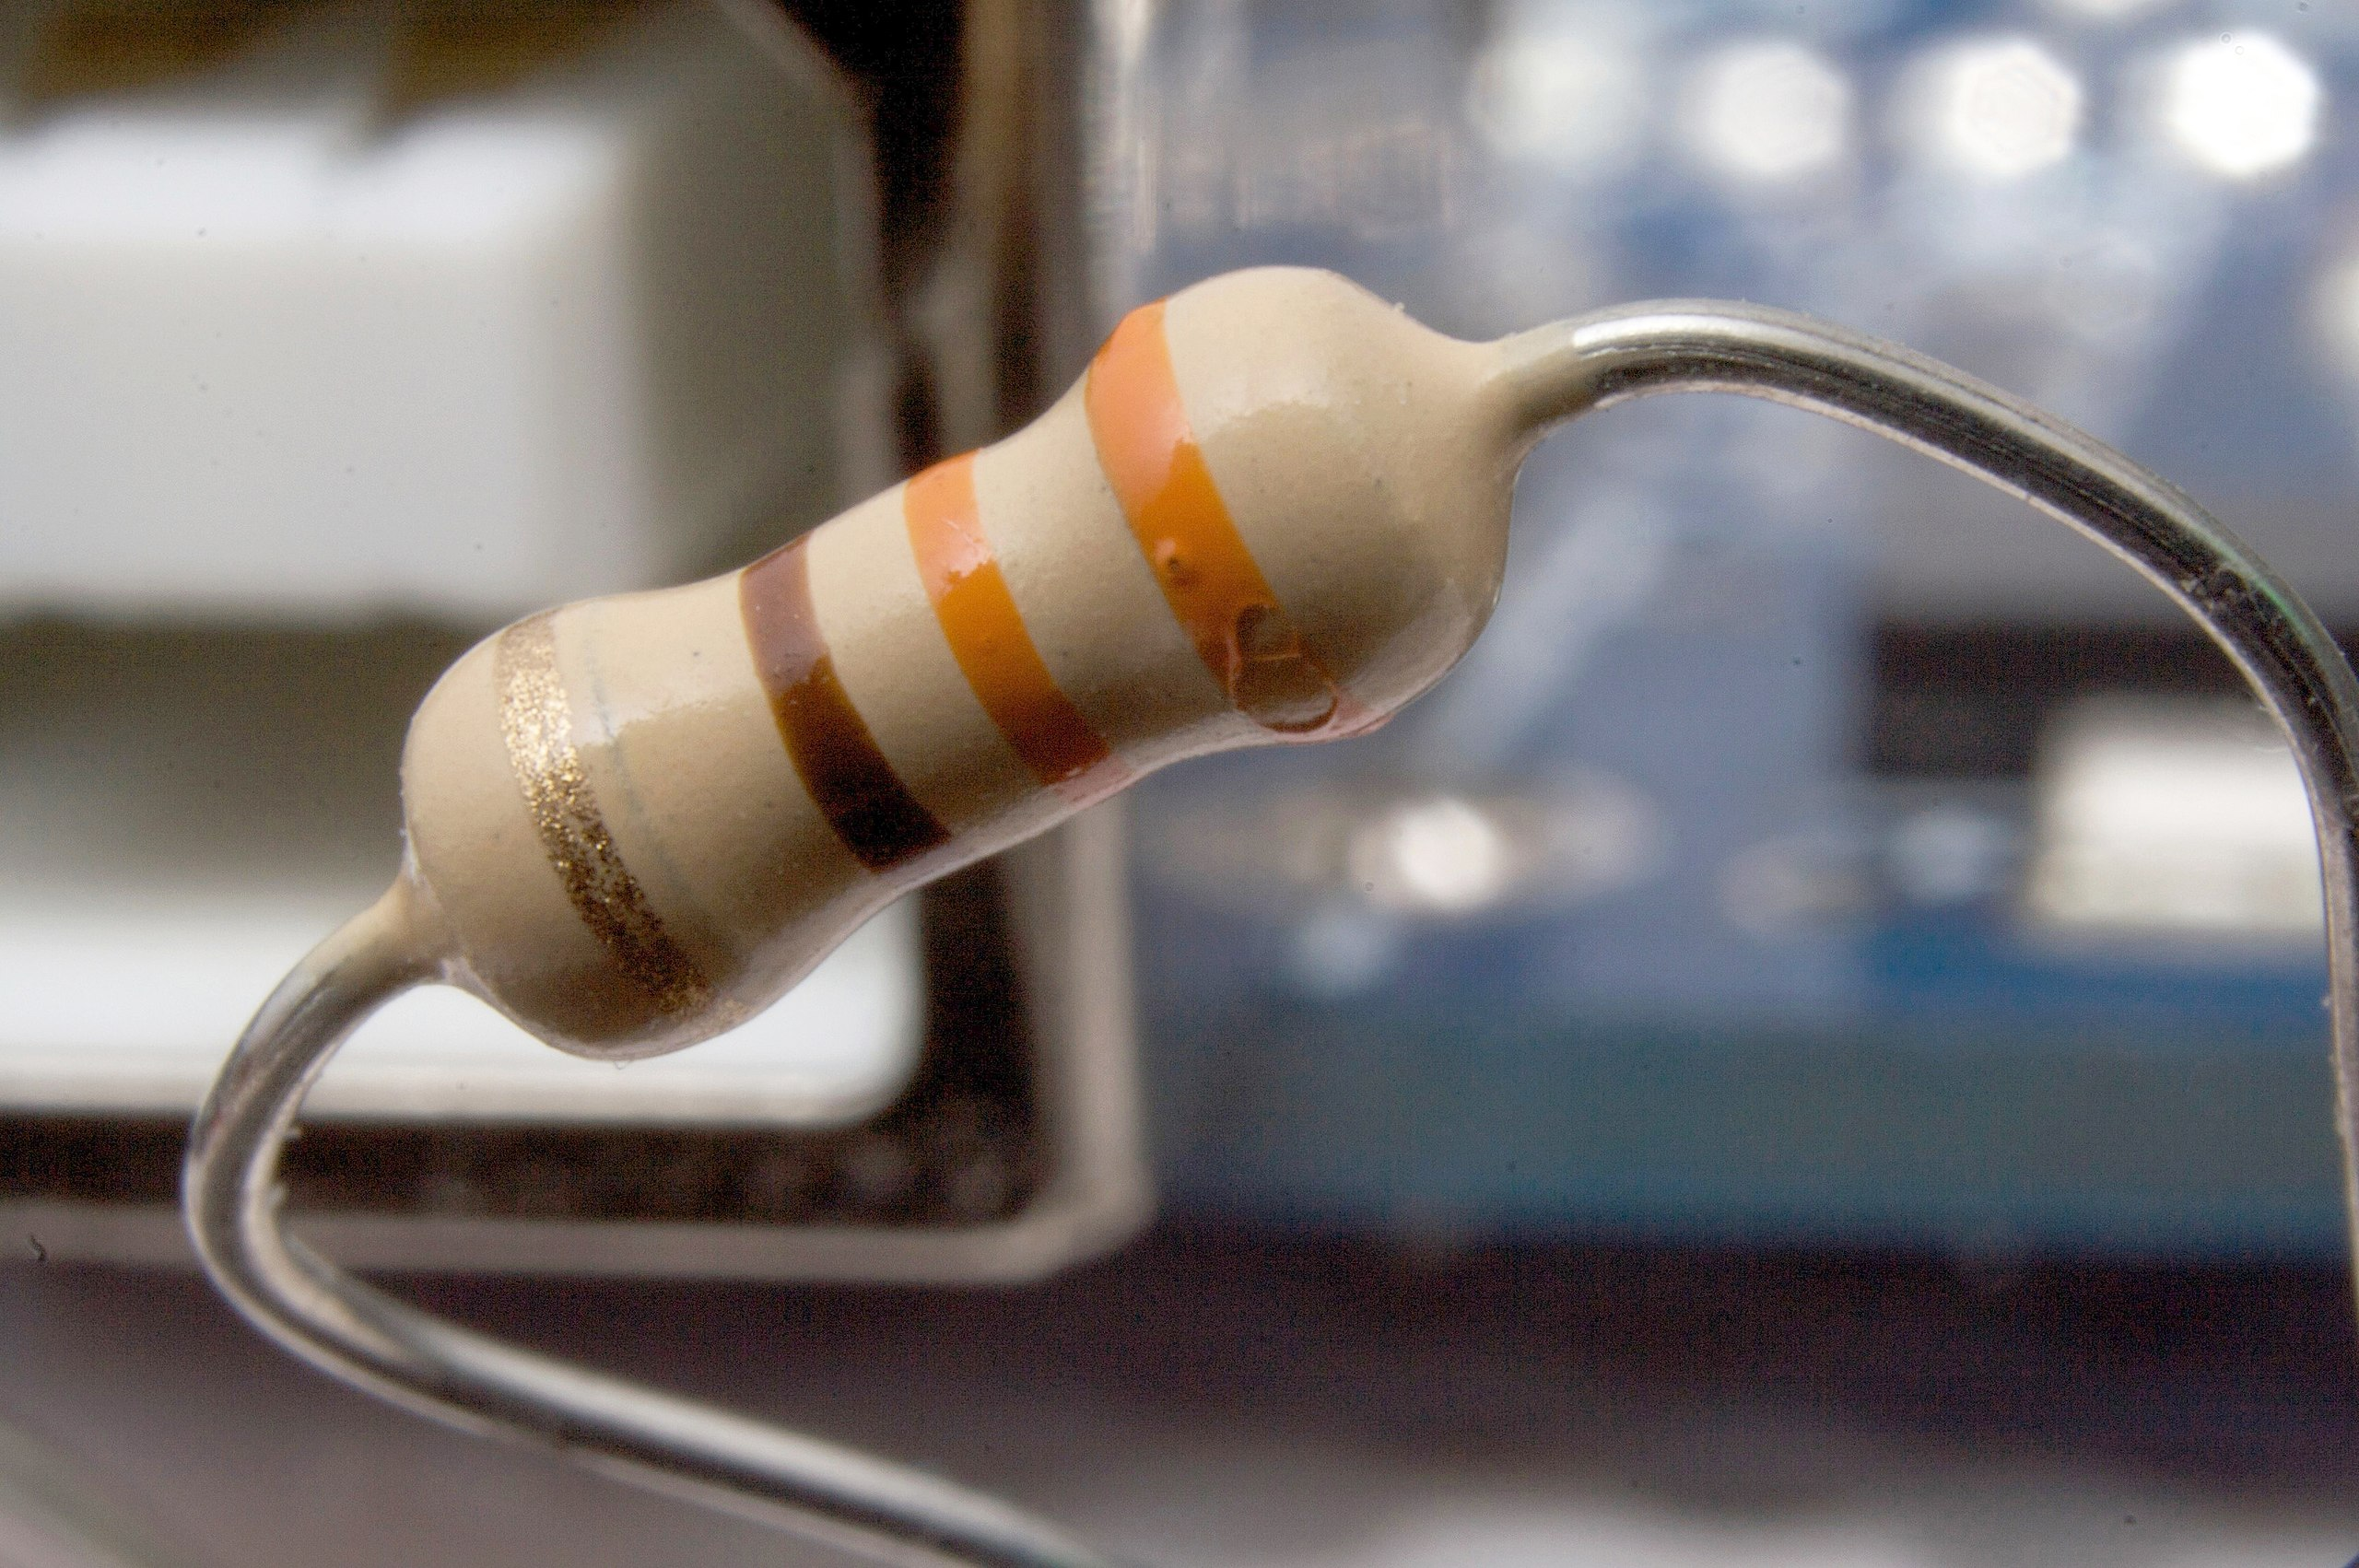
\includegraphics[width=0.4\textwidth]{resistor.jpg}
  \end{center}
  \caption{\label{fig:data}330\ohm \hspace{0.2cm}Axial-lead resistor.}
\end{wrapfigure}

These are high \textbf{resistance} (R) systems, as they're severely limiting the current (or flow of people out of the elevator). Conversely, maybe the elevator's doors open extremely wide or everyone just falls through a trap door at the bottom. These would be low resistance systems, as they permit higher flow rates.

Sometimes it's beneficial to have a higher resistance system. By reducing the quantity of charge leaving the system, that energy can be saved for a later use. Other times, it's nice to use that energy more quickly. In that case, a lower resistance is desired.
The relationship between the Voltage and the Current of the system is defined by the very simple Ohm's law:
\begin{equation} \label{eq:ohm}
V = IR
\end{equation}

\subsection{Power}
The \textbf{power} of a system is is the amount of work that system does per unit of time. In an electrical system, the equation for power is:

\begin{equation} \label{eq:power}
P = VI
\end{equation}

\vspace{0.2cm}
Using Ohm's law, it's possible to rewrite the system in a couple  of ways: $P=V^2/R$, $P=I^2R$. In most systems (especially resistors), the power loss will be primarily heat loss. Every component has a maximum \textit{power rating}, going beyond which will destroy the component. Sometimes (like in air heaters), we want components to be able to convert electrical energy into heat and dissipate that effectively. We'd expect these systems to have lower resistance or higher voltages.

\subsection{Ground / GND}

\begin{figure}[!b]
  \begin{center}
    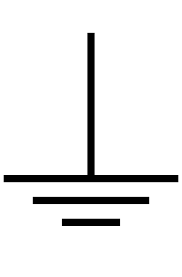
\includegraphics[width=0.2\textwidth]{gnd.png}
  \end{center}
  \caption{\label{fig:gnd}Common symbol for ground (GND).}
\end{figure}

While anything outside of a pure vacuum will have atomic activity, it's convenient to introduce the idea of the \textbf{ground} state as an empty space that is the most attractive possible region for electrons. Because it is so attractive, the electrons will take any possible path to reach this ground state. The successful movement of electrons from the excited state to the ground state is often referenced as a loop. Another point of note about ground is that it's an infinitely large reservoir. That is, dumping as many charged particles as you like into this reservoir will not increase the overall charge of ground.

\newpage

\subsection{Capacitance}

\begin{wrapfigure}{r}{0.4\textwidth}
  \begin{center}
    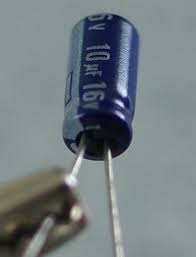
\includegraphics[width=0.25\textwidth]{electrolytic_cap.jpeg}
  \end{center}
  \caption{\label{fig:electrlytic}Electrolytic.}
\end{wrapfigure}

A good analogy for capacitors is a rubber band. These little devices hold charge and can quickly release it if needed. Let's dissect the governing equation behind them:

\begin{equation} \label{capacitance}
I(t) = C\frac{dV(t)}{dt}
\end{equation}

\vspace{0.2cm}
The current (I) is related to some term "C" and the rate of change of the voltage. This means that when there is a high current through the system, the voltage across the capacitor is changing rapidly. Likewise, if the voltage is not changing, then there is no current in the system. Integration of this equation gives even more clues:

\begin{equation} \label{eq:capacitance_init}
V(t) = \frac{\int I(t)dt}{C}+V_o(t)
\end{equation}
\vspace{0.2cm}

Assuming {$V_o(t) = 0$}, the output voltage ("electric pressure", or $V(t)$) is proportional to the amount of charged particles that entered the system. You can think of this as a sort of reactance to change, just like the rubber band's reluctance to being pulled. These properties of capacitors make them particularly useful for smoothing out peaks in voltage lines (AC to DC) and for building oscillators.

\subsection{Inductance}
\begin{wrapfigure}{r}{0.4\textwidth}
  \begin{center}
    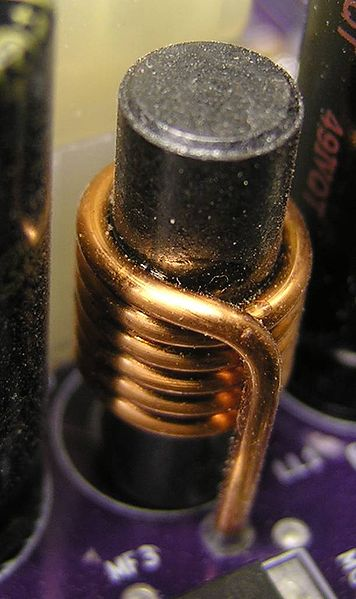
\includegraphics[width=0.25\textwidth]{inductor.jpg}
  \end{center}
  \caption{\label{fig:data}Inducting Coil.}
\end{wrapfigure}

One of the neatest electrical components but also one of the more advanced, inductance is another way of storing energy. Have you ever tried to make a whirlpool in the pool with a few other people? It's challenging at first, but once you get the water moving it's almost effortless to keep moving in a circle and in fact you can let the water carry you at times. When current moves in a circle, it opposes the magnetic field in a similar way that your body opposes the water. The relationship between voltage (in this case effort required to start the whirlpool) and current (the speed of the whirlpool) is described by this equation:

\begin{equation} \label{eq:inductance}
V(t) = L\frac{dI(t)}{dt}
\end{equation}
\vspace{0.2cm}

Bringing this back to our whirlpool example, this equation can help explain some of our intuition. If you don't want to change the current {$\frac{dt(t)}{dt} = 0$}, then no effort is require. This is true if there's a raging vortex or if there's no whirlpool at all. Conversely, changing the current requires an effort proportional to how much the current is changing. If we put a big wall down into the middle of a vortex, it will experience a large force on its face the instant we put it into the vortex. This is due to the significant change in current as the water goes from full motion to full stop.
\newpage

\section{Circuit Design Tools}
\subsection{Kirchhoff’s Voltage Law (KVL)}

\begin{wrapfigure}{r}{0.4\textwidth}
  \begin{center}
    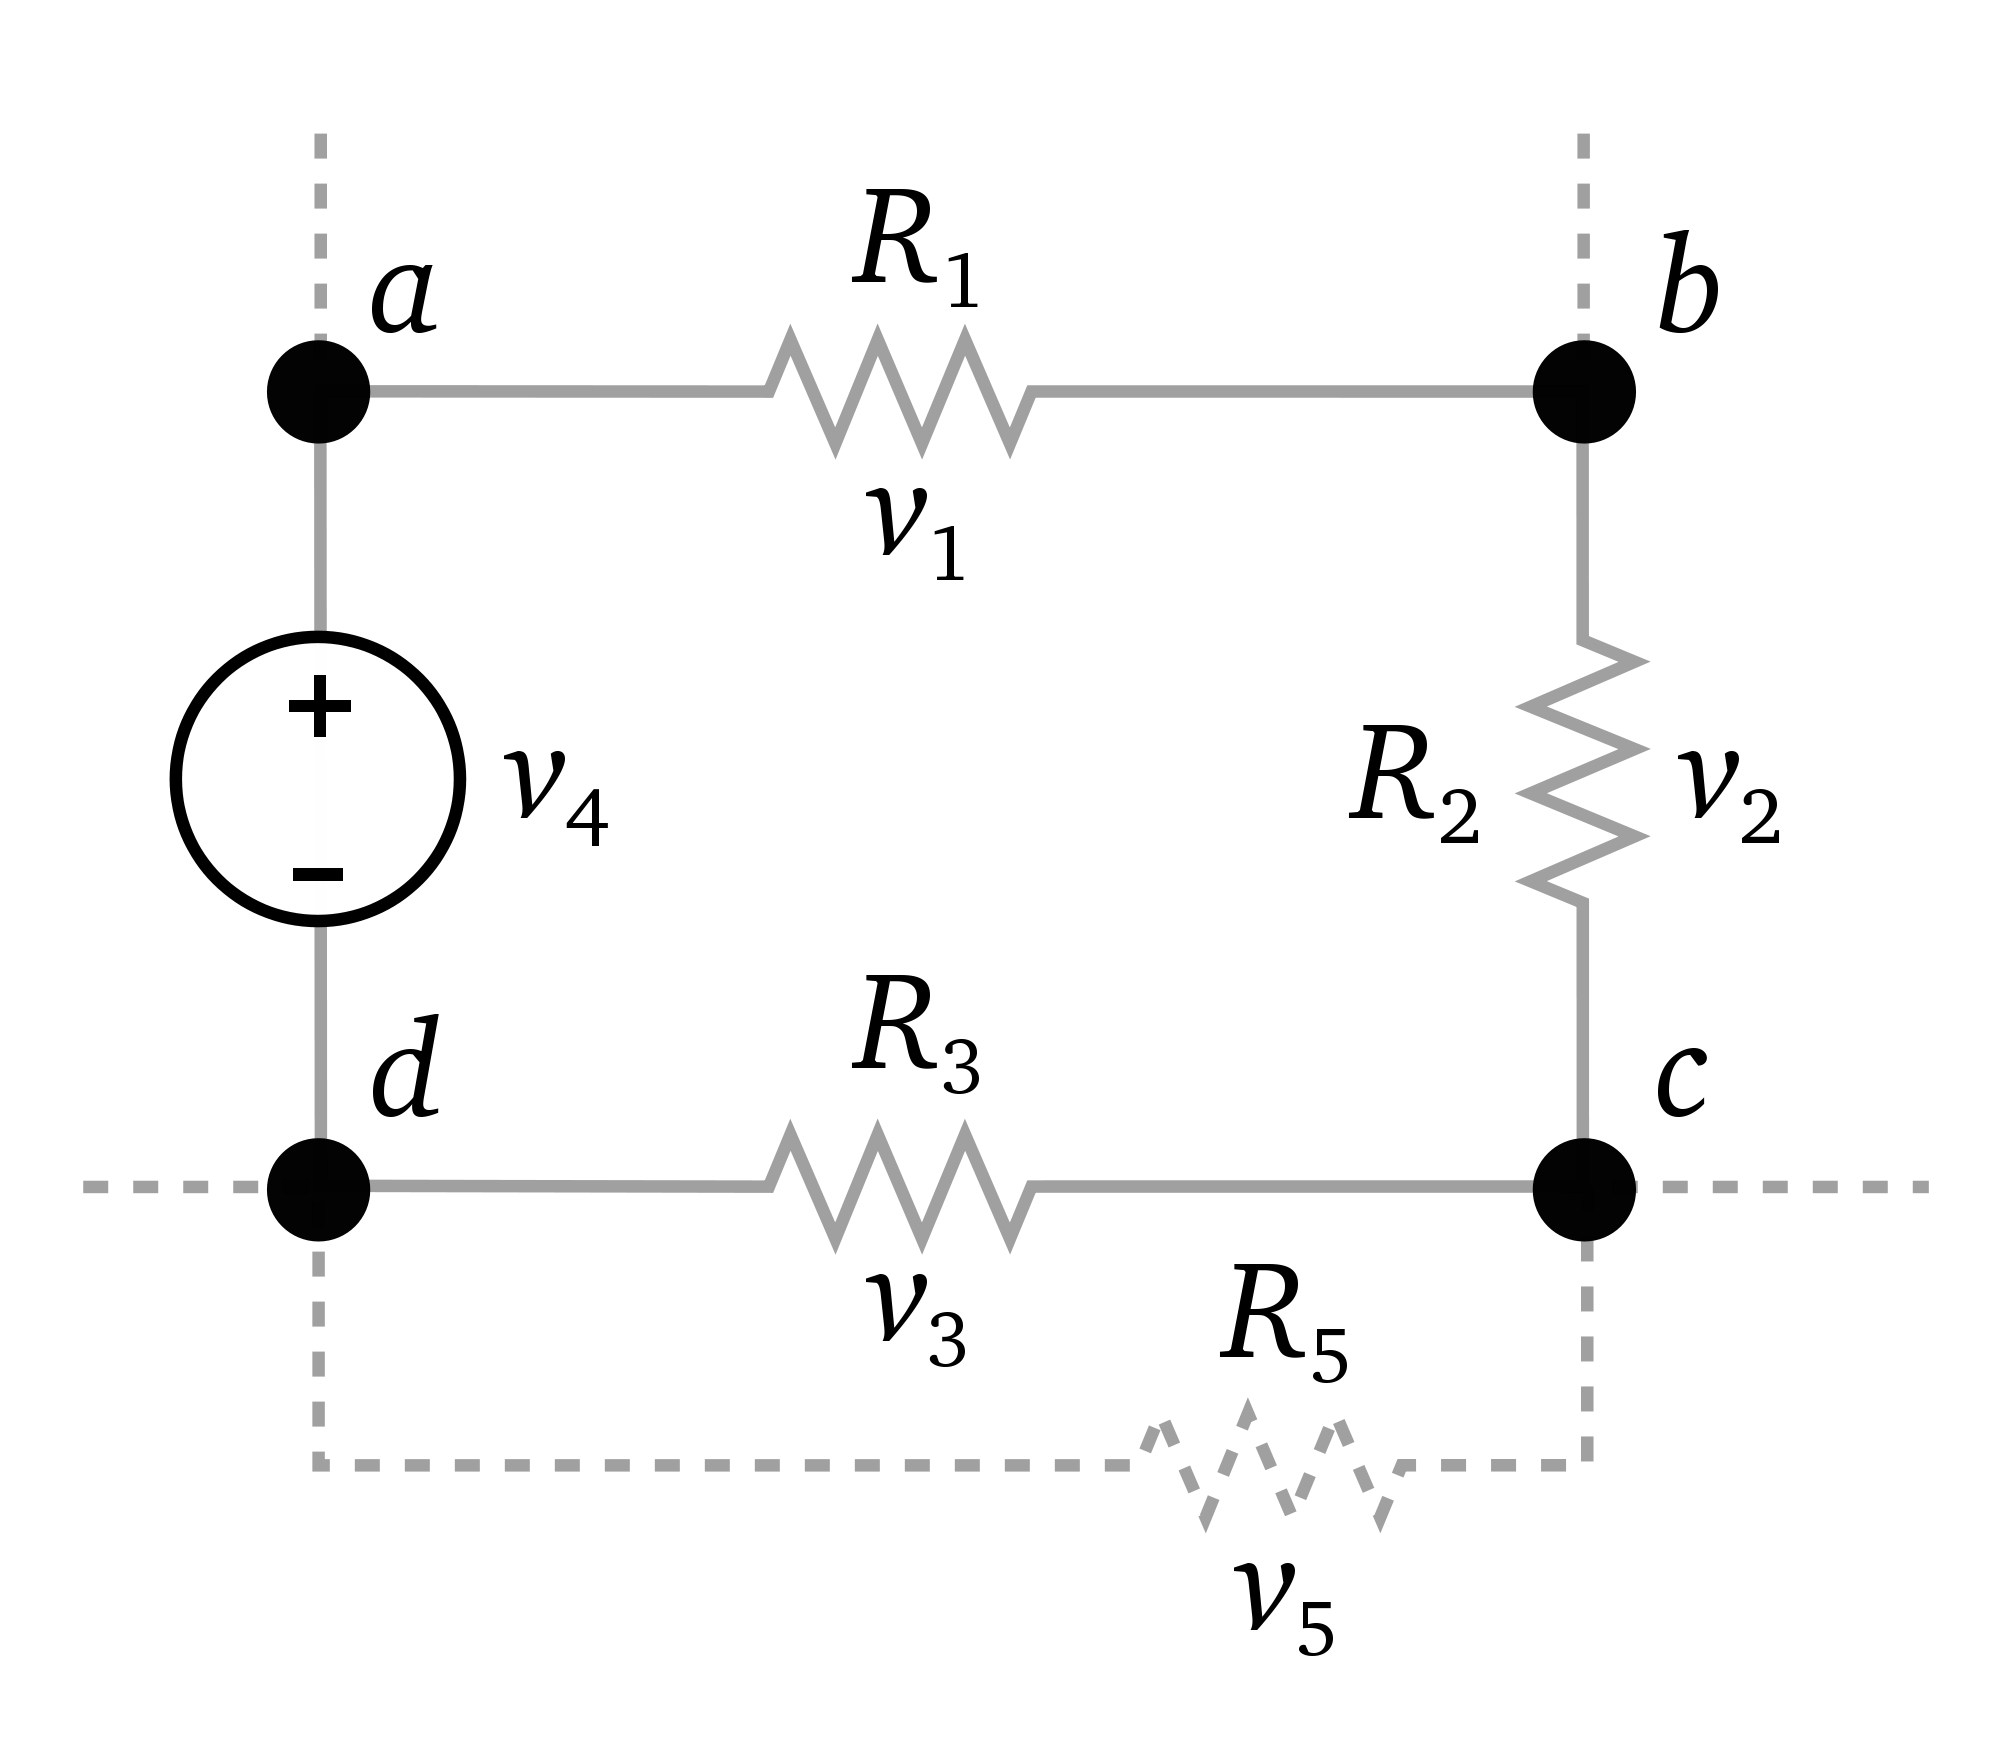
\includegraphics[width=0.35\textwidth]{kvl.png}
  \end{center}
  \caption{\label{fig:kvl}Kirchhoff’s Voltage Law.}
\end{wrapfigure}

One of the most common tools in circuit analysis is Kirchhoff’s Voltage Law (KVL). This tells us that the sum of voltages around any loop will equal zero. If we use the metaphor of a staircase (where the top of the staircase is high voltage and the bottom is the ground), then this would be saying that the height of the total staircase is the sum of the heights of each individual step. So obvious we shouldn't even have to say it, right? In this way, we could imagine ourselves standing on the group, appropriately connected to Ground (GND). Any ascent would be a contribution in the positive voltage path, and any descent would be a negative contribution. But at the end of the day, there's a clear path to get between each of these altitudes.

Thus, if we have a circuit with a battery and three resistors (Fig \ref{fig:kvl}), the voltage is across the battery (think climbing a ladder) plus the sum of the voltages across the three resistors (climbing back down three stairs - this is a negative contribution) would equal zero. Therefore each resistor will carry a certain amount of the load of the battery's voltage.

\vspace{0.5cm}
\noindent
\textbf{NOTE:} an important point of note is that when paired with Ohm's Law \eqref{eq:ohm}, this tells us the voltage drop across each unit of resistance within the system, and that the specific voltage drop across one resistor is directly related to its contribution to the system resistance.

\subsection{Kirchhoff's Current Law (KCL)}

\begin{wrapfigure}{r}{0.4\textwidth}
  \begin{center}
    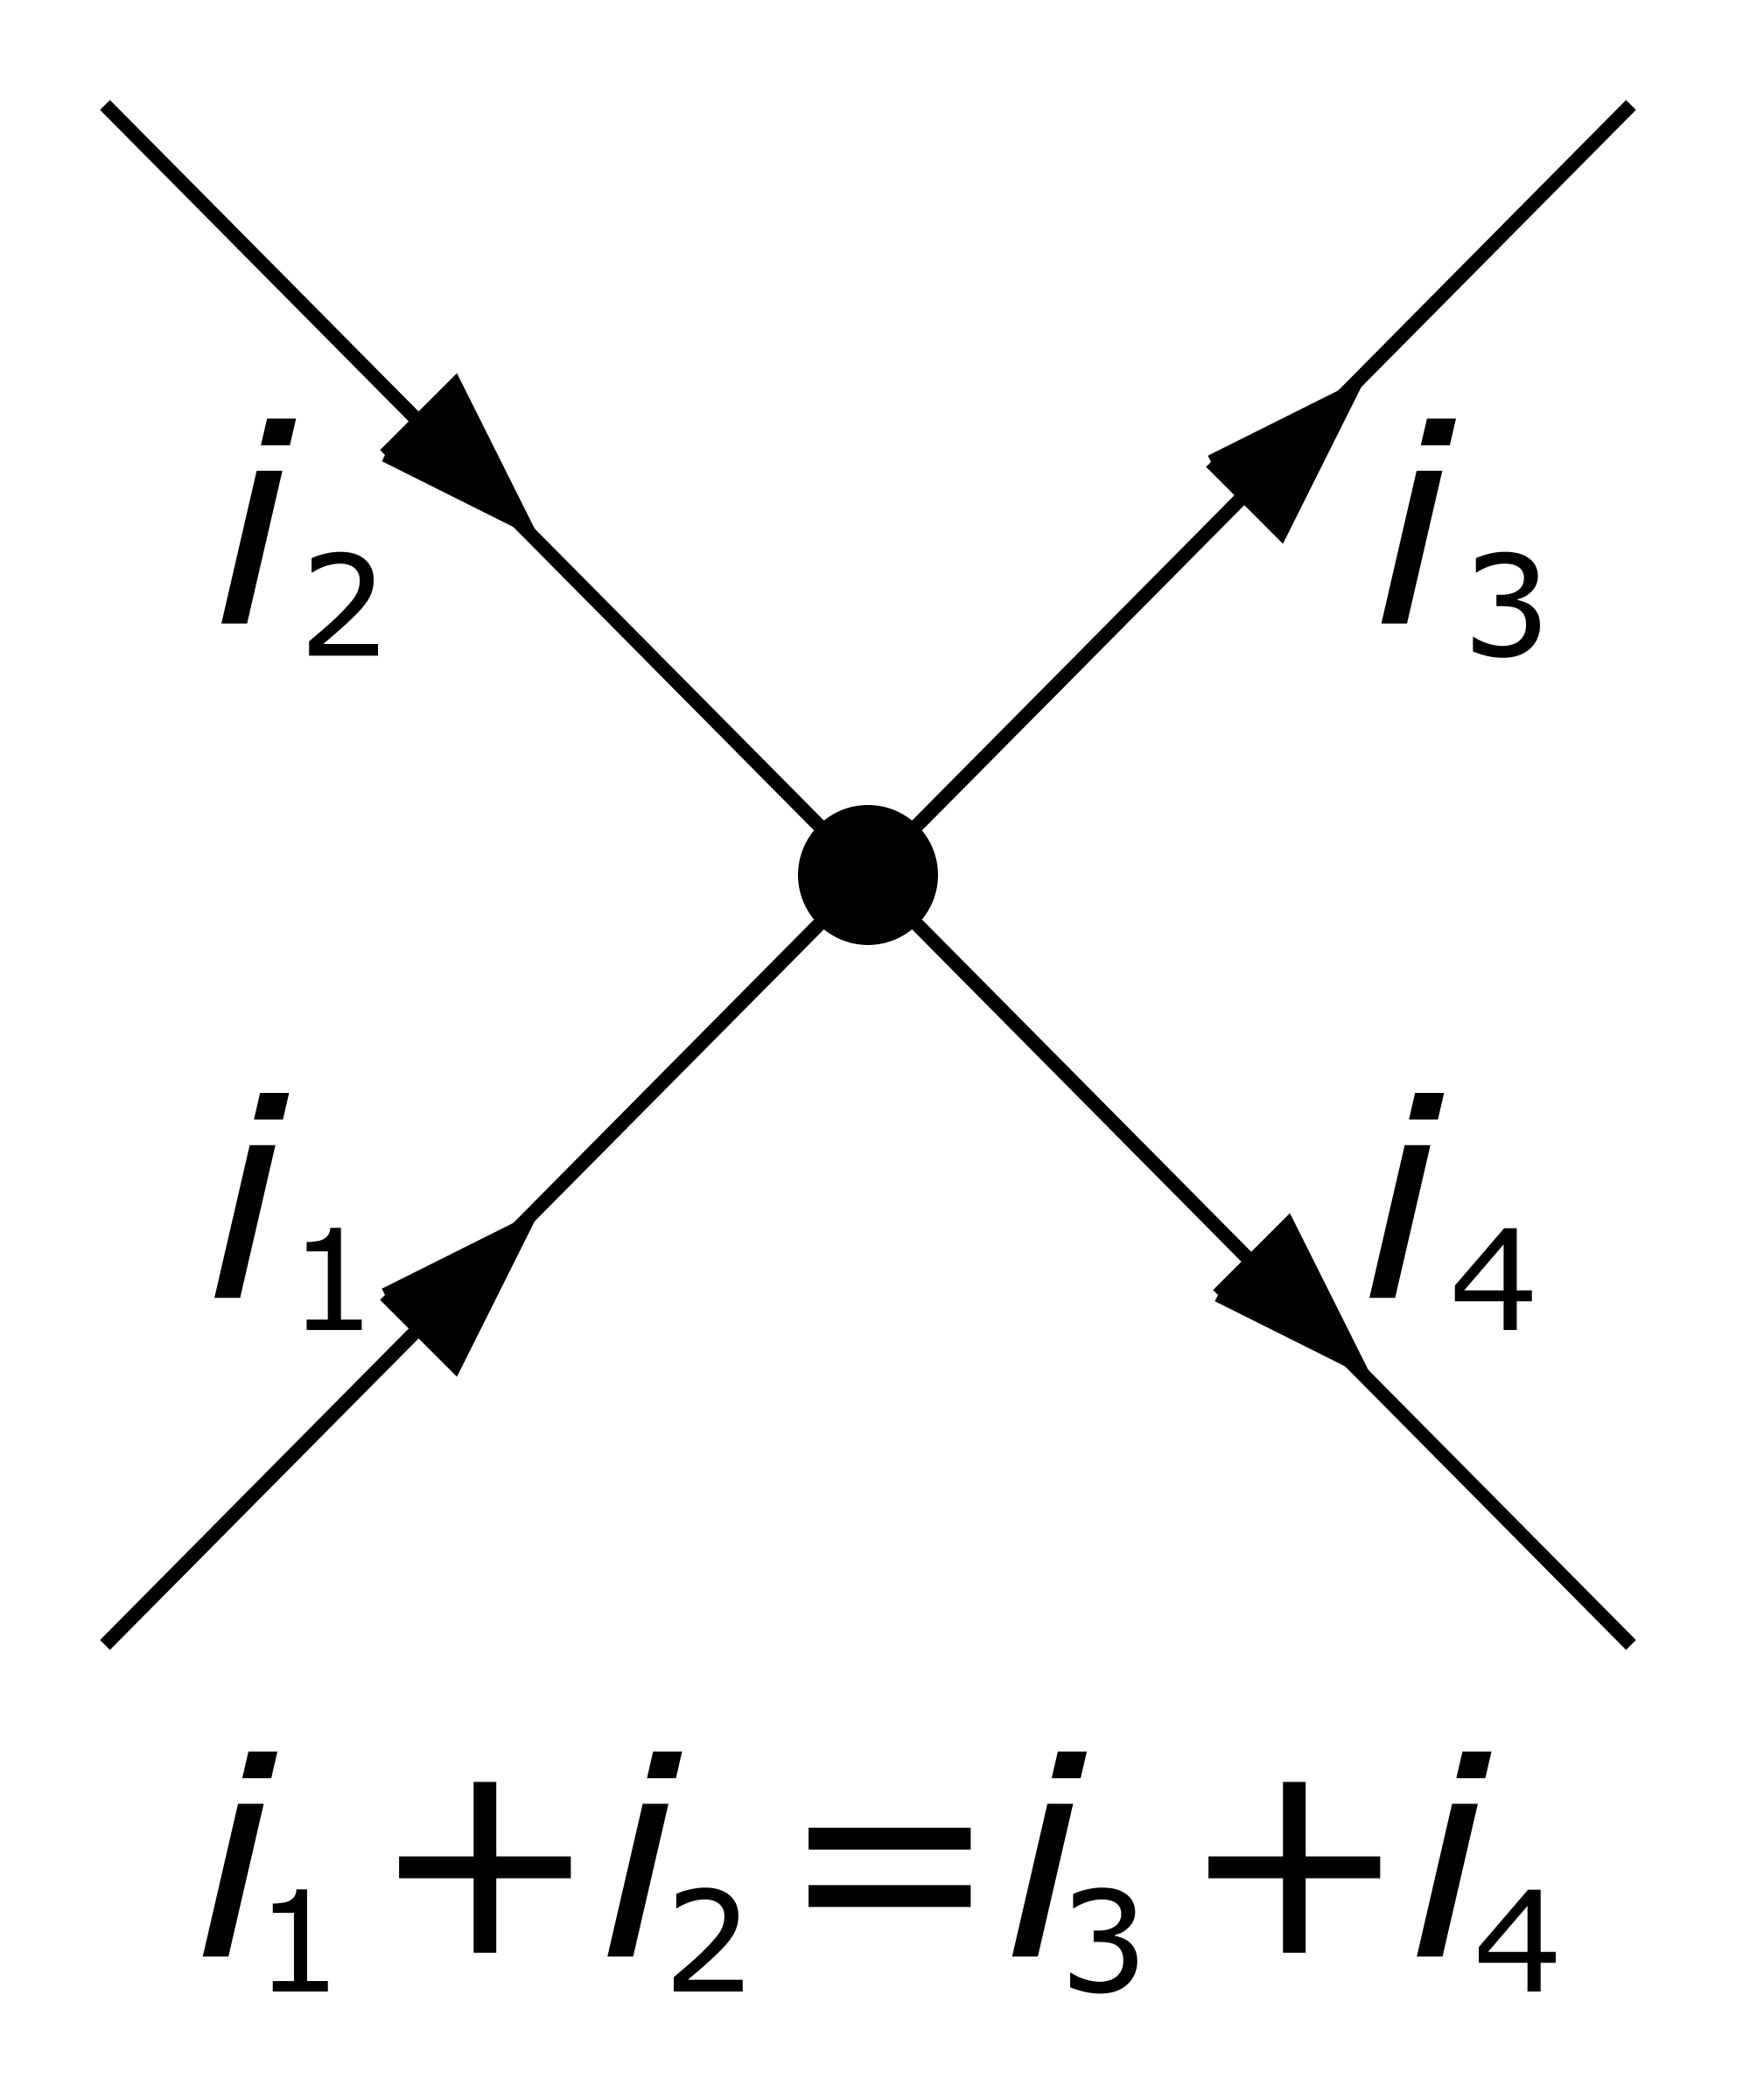
\includegraphics[width=0.35\textwidth]{kcl.png}
  \end{center}
  \caption{\label{fig:kvl}Kirchhoff’s Current Law.}
\end{wrapfigure}

Kirchhoff's Current Law (KCL) is likewise extremely simple when applied to a physical phenomena. Instead of thinking about voltage, this law applies to current. As such, we use the metaphor of a river instead of a hill. In this example, our current is synonymous with that of water flowing. This law is saying that at any given point in our metaphoric "river", the water coming into the system must be equal to the water going out of the system. This is interesting when the river splits into two tributaries, as more of the water flows in one direction and less in another. What our KCL law tells us though is that the water leaving the system is equal to the water entering. Therefore even if the river splits, we know that the volume of water leaving through the two tributaries is equal to the volume of water coming in.

\vspace{4cm}
\noindent

\newpage
\section{Exercises}
Q1 - What is the voltage at X? What's the voltage after the 4.7k resistor is removed?

\begin{figure}[h!]
\centering
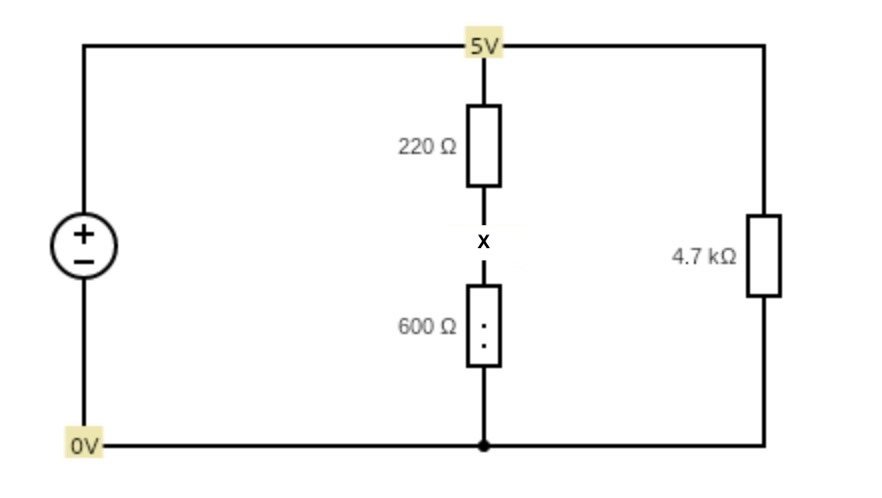
\includegraphics[width=0.7\textwidth]{q1.jpg}
\caption{\label{fig:data}Voltage Divider 1.}
\end{figure}

\begin{figure}[h!]
\centering
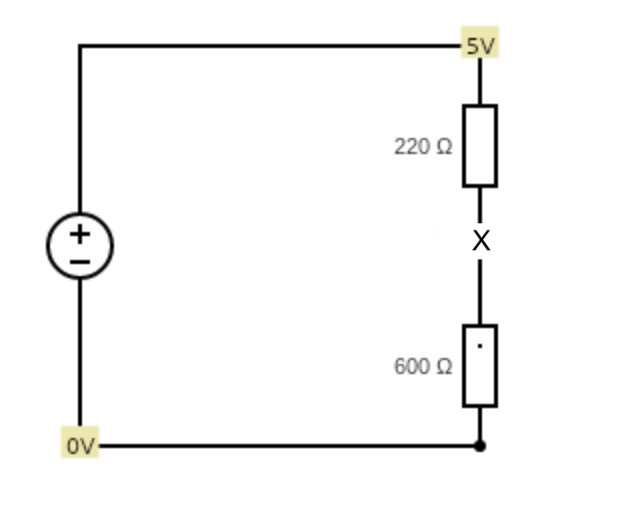
\includegraphics[width=0.5\textwidth]{q2.jpg}
\caption{\label{fig:data}Voltage Divider 2.}
\end{figure}

\newpage
\noindent
Q2 - What is the voltage at Vout, in terms of  $R_{1}$, $R_{2}$, $R_{3}$, and $R_{4}$?

\begin{figure}[h!]
\centering
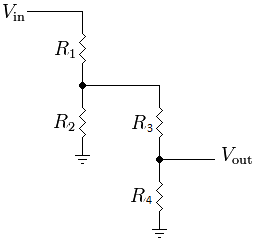
\includegraphics[width=0.5\textwidth]{q3.png}
\caption{\label{fig:data}Voltage Divider 2.}
\end{figure}


\newpage
\section{Learn More}
\noindent
Check out this resource to get a better idea of how a capacitor charges and discharges:
\href{https://www.falstad.com/circuit/}{falstad.com/circuit/}

\vspace{0.5cm}
\noindent
For more theory on electricity and magnetism, this physics text by Hans C. Ohanian should give you a great starting point: \cite{9780393930047}

\vspace{0.5cm}
\noindent
All of the equations and theory from this module are from Hambley's Electrical Engineering text \cite{9780133116649}, which is an excellent introduction to more thorough electrical engineering practices.

\vspace{0.5cm}
\noindent
Diving into hobbyist projects are a great way to get started applying a lot of these core ideas, so pick up an Arduino and go build something cool! This YouTuber offers a lot of great projects and theory guides, I highly recommend his videos to start: \href{https://youtu.be/BtLwoNJ6klE}{youtu.be/BtLwoNJ6klE}.

\bibliographystyle{unsrt}
\bibliography{references.bib}

\end{document}